\documentclass{article}
\usepackage{booktabs}
\usepackage{tabularx}
\usepackage{float}
\usepackage{graphicx}
\usepackage{geometry}
\geometry{margin=1in}
\begin{document}

\section*{Moda de Evaluaciones en Reexplicaciones}

\begin{table}[H]
\centering
\caption{Valor más frecuente por campo}
\begin{tabularx}{0.7\textwidth}{lX}
\toprule
\textbf{Campo} & \textbf{Moda} \\
\midrule
Fidelidad & alta \\
Simplificacion & alta \\
Alucinacion & False \\
\bottomrule
\end{tabularx}
\end{table}

\begin{figure}[H]
\centering
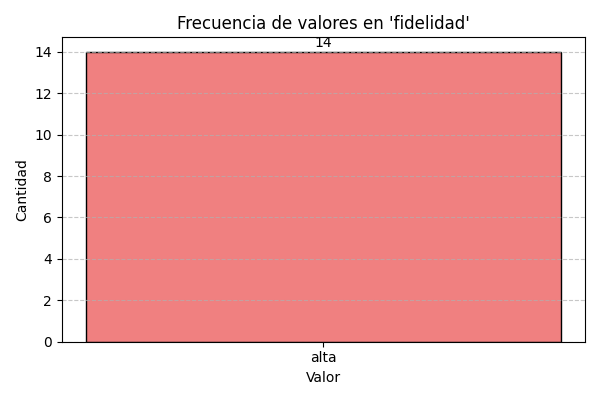
\includegraphics[width=0.8\textwidth]{../graficos/fidelidad_frecuencias.png}
\caption{Frecuencia de valores para fidelidad}
\end{figure}

\begin{figure}[H]
\centering
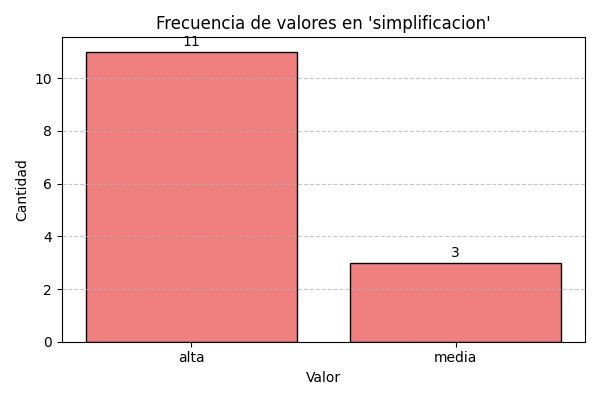
\includegraphics[width=0.8\textwidth]{../graficos/simplificacion_frecuencias.png}
\caption{Frecuencia de valores para simplificacion}
\end{figure}

\begin{figure}[H]
\centering
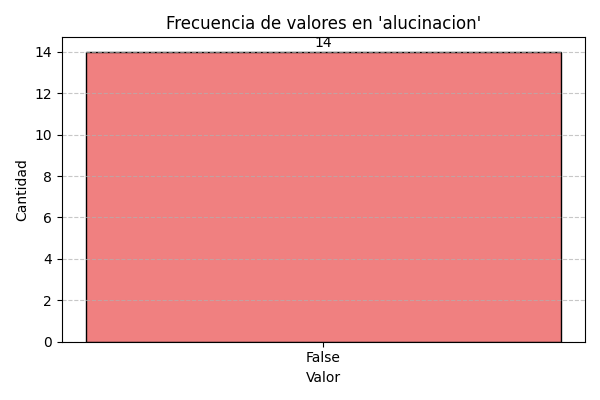
\includegraphics[width=0.8\textwidth]{../graficos/alucinacion_frecuencias.png}
\caption{Frecuencia de valores para alucinacion}
\end{figure}
\end{document}